\chapter{parxpaMcada atuyxnanxta maTaTxda vijAcnxni AyaRBaTa}%%%2

halavAru hosa parxyoVgagaLanunx, halavu mUla aBipArxyagaLanunx parxpaMcakekx modala bAri koTaTx BAratiVya budidhxvaMta sherxVSaThxru kirx.sha.~{\rm 400} riMda {\rm 1200}ra varegina sumAru {\rm 800} vaSaRgaLa avadhiyalilxdadx meVdhAvigaLu.

kirx.sha.~{\rm 5}neV shatamAnadiMda kirx.sha. {\rm 7}neya shatamAnadavaregina kAlavanunx BAratiVya KagoVla matutx gaNita shAsatxrXgaLa savxNaRyuga eMdu kelavaru aBipArxya paDutAtxre.

kirx.sha.~{\rm 5}neV shatamAnadalilxdadx kusumApurada AyaRBaTa, {\rm 6}neya shatamAnada varAhamihira matutx {\rm 7}neV shatamAnada barxhamxgupatx matutx modalaneya BAsakxra ivaralilx muKayxru.

gaNita matutx KagoVla vijAcnxnagaLige oMdu vayxvasithxta hAgU vaYjAcnxnika mAgaRvanunx toVrisikoTaTx kiVtiR hAgU gaNita matutx KagoVlajacnxra aneVka AviSAkxragaLige modaliga eMba kiVtiRyU AyaRBaTarige salulxtatxde.

parxpaMcada sherxVSaThxmaTaTxda vijAcnxnigaLa peYki kirx.sha. {\rm 499}ralilx `AyaRBaTiVyaM' bareda BAratiVya gaNitajacnx hAgU KagoVla tajacnx AyaRBaTarU obabxru.

AyaRBaTiVyadalilx Eka ({\rm 1}), dasha ({\rm 10}), shata ({\rm 100}), sahasarx ({\rm 1000}), Ayuta ({\rm 10,000}), niyuta ({\rm 1,00,000}), parxyuta ({\rm 10,00,000}), koVTi ({\rm 1,00,00,000}), nayxbuRda athavA nUru koVTi - iMtha dashamAna padadhxti tiLisuva {\rm 18} sAthxnagaLu gurutisalapxTiTxve.

\newpage

AyaRBaTaru gaNita, kAlakirxyA, goVlamf eMba mUru BAgagaLanunx tananx garxMtha `AyaRBaTiVyaM'nalilx parxsAtxpisidAdxre.

AyaRBaTaru viShayagaLanunx nAlukx pAdagaLAgi viBAgisidAdxre.
\begin{itemize}
\item[{\rm 1)}] {\bf giVtikApAda:} idaralilx {\rm 13} sholxVkagaLive. idaralilx KagoVla vijAcnxnakekx saMbaMdhisida kelavu muKayxvAda bele matutx lekAkxcAragaLanunx sUtarxda rUpadalilx koDalAgide.

\item[{\rm 2}] {\bf gaNitapAda:} idaralilx {\rm 33} sholxVkagaLive. idaralilx vagaRmUla, GanamUla tiBujada keVtarxPala (sale), vaqtatxda sale, sherxVDhiV gaNita, vagaRsamiVkaraNa, kuTaTxka matutx vagaR, anidiRSaTx samiVkaraNagaLu, shaMkuvina neraLugaLa lakekxgaLu, terxYrAshi muMtAda viSayagaLa bagegx vivaraNeyide. 
  
\item[{\rm 3}] {\bf kirxyApAda:} idaralilx {\rm 25} kArikegaLive. idaralilx kAlada viBAgagaLu sUyaR, caMdarx matutx itara garxhagaLa sAthxnagaLa niSakxsheR, vividha mAsa saMvatasxragaLu muMtAda viSayagaLive.
 
\item[{\rm 4}] {\bf goVlAdhAyxya:} idaralilx $50$ kArikegaLive. idaralilx BUmi guMDAgiruvudu. adu parxtidina tananx akaSxda sutatxlU tirugutitxruvudariMda sUyoVRdaya, sUyARsatxgaLu uMTAgutitxruvudu. BUmi matutx itara garxhagaLu savxyaM parxkAsha vasutxgaLalalx, BUmi pashicxmadiMda pUvaRda kaDege tirugutitxde I parxsAtxpagaLelalx ive.
  \end{itemize}


\noindent
{\bf KagoVlavijAcnxnakekx AyaRBaTara mahatavxda koDugegaLeMdare.}

\begin{itemize}
\item[{\rm 1)}] BUmiya AkAra matutx calane
  
\item[{\rm 2)}] sUyoVRdaya matutx sUyARsatx beVre beVre jAgagaLalilx beVre beVre kAlakekx uMTAgutatxve.
  
\item[{\rm 3)}] BUmiya utatxra dhurxva matutx dakiSxNa dhurxva parxdeVshagaLalilx Aru tiMgaLu hagalu matutx Aru tiMgaLu rAtirx irutatxve.

\item[{\rm 4)}] mahAyugaveMba oMdu diVGaRkAlavadhiyalilx oMdoMdu AkAshakAya eSeTxSuTx pariBarxmaNegaLanunx pUtiRyAgi mugisutatxde eMba saMKeyxgaLanunx koTiTxdAdxre. mahAyugada badalu kalapx eMba shabadx parigaNisi A avadhiyalilx garxhagaLa pariBarxmaNa saMKeyxgaLanUnx niVDidAdxre. 

\item[{\rm 5)}] saMparxdAyadiMda baMdidadx yuga sidAdhxMtavanunx biTuTx sulaBavAda matutx garxha gaNitada lekAkxcAragaLige anukUlavAguva hosa riVtiya yuga viBajaneyanunx yoVcisidAdxre. 

\item[{\rm 6)}] eraDu garxhagaLu edurubadurAgi calisutitxdadxre A eraDara aMtaravanunx avugaLa veVgagaLa motatxdiMda BAgisi, oMdeV dikikxnalilx calisutitxdadxre avugaLa aMtaravanunx veVgagaLa vayxtAyxsadiMda BAgisidare Aga baruva BAgalabadhxvu A eraDu garxhagaLu saMdhisuva athavA saMdhisada
\begin{figure}[H]
\centering
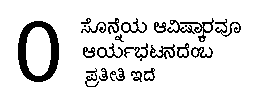
\includegraphics{src/figures/fig17.eps}
\end{figure}
  naMtarada kAlAvadhiyanunx koDutatxde.
  
\item[{\rm 7)}] oMdu mahAyugada kAlAvadhiyalilx, BUmiyiMda viVkiSxsidAga sUyaR, caMdarx, garxhagaLu eSeTxSuTx pariBarxmaNegaLanunx mugisutatxve eMbudanunx koTiTxdAdxre. 

\item[{\rm 8)}] caMdarxgarxhaNa matutx sUyaRgarxhaNagaLu saMBavisalu veYjAcnxnika kAraNagaLanunx suPxTavAgiyU, saMkeSxVpavAgiyU tiLisidAdxre. 
  
\item[{\rm 9)}] sUyaR caMdArxdigaLa suPxTa sAthxnagaLanunx viVkAsxNeyiMda tALe noVDalu saMkiSxpatxvAgi heVLidAdxre. (AdhArita)
\end{itemize}
